% Created 2025-04-27 Sun 22:34
% Intended LaTeX compiler: pdflatex
\documentclass[11pt]{article}
\usepackage[utf8]{inputenc}
\usepackage[T1]{fontenc}
\usepackage{graphicx}
\usepackage{longtable}
\usepackage{wrapfig}
\usepackage{rotating}
\usepackage[normalem]{ulem}
\usepackage{amsmath}
\usepackage{amssymb}
\usepackage{capt-of}
\usepackage{hyperref}
\usepackage{minted}
\usepackage[polish]{babel}
\usepackage[margin=1cm]{geometry}
\usepackage{float}
\usepackage{siunitx}
\author{Emil Siatka, Marek Swakoń, Patryk Górski, Piotr Pich}
\date{Data oddania: 03.04.2025}
\title{Ćwiczenie 1.}
\hypersetup{
 pdfauthor={Emil Siatka, Marek Swakoń, Patryk Górski, Piotr Pich},
 pdftitle={Ćwiczenie 1.},
 pdfkeywords={},
 pdfsubject={},
 pdfcreator={Emacs 30.1 (Org mode 9.7.11)}, 
 pdflang={Polish}}
\begin{document}

\maketitle
\tableofcontents

\section{Wprowadzenie}
\label{sec:org91ad8a8}

Celem ćwiczenia jest zaprojektowanie bazującego na bramkach NAND układu kombinacyjnego
realizującego transkoder trzybitowej liczby binarnej na układ graficzny emotikony wyświetlanej na
szesnastu punktach, zgodnie z rysunkiem 1.

\begin{figure}[H]
\centering
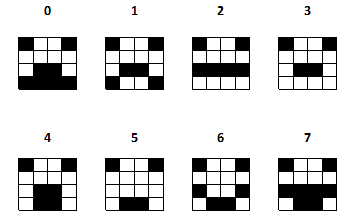
\includegraphics[width=.9\linewidth]{rys1.png}
\caption{Docelowe wyniki działania transkodera}
\end{figure}

Interfejs układu będzie wyglądał wówczas identycznie do podukładu na rysunku 2.

\begin{figure}[H]
\centering
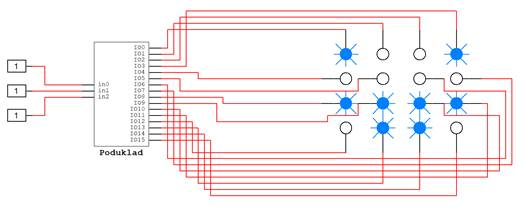
\includegraphics[width=.9\linewidth]{rys2.jpg}
\caption{Interfejs projektowanego układu}
\end{figure}

Projektowany układ przedstawić możemy jako układ którego sygnałami wyjściowymi jest 16 trójargumentowych funkcji zdaniowych \(P_0, P_1, \cdots, P_{15}\)
(gdzie każdy punkt wyświetlacza odpowiada wynikowi jednej funkcji) przyjmujących poniższe wartości:

\begin{table}[H]
\caption{Tabela prawdy dla funkcji \(P_0, P_1, \cdots, P_{15}\)}
\centering
\begin{tabular}{|c|c|c|c|c|c|c|c|c|c|c|c|c|c|c|c|c|c|c|c|}
\hline
\(A\) & \(B\) & \(C\) &  & \(P_0\) & \(P_1\) & \(P_2\) & \(P_3\) & \(P_4\) & \(P_5\) & \(P_6\) & \(P_7\) & \(P_8\) & \(P_9_{}\) & \(P_{10}\) & \(P_{11}\) & \(P_{12}\) & \(P_{13}\) & \(P_{14}\) & \(P_{15}\)\\
\hline
0 & 0 & 0 &  & 1 & 0 & 0 & 1 & 0 & 0 & 0 & 0 & 0 & 1 & 1 & 0 & 1 & 1 & 1 & 1\\
0 & 0 & 1 &  & 1 & 0 & 0 & 1 & 0 & 0 & 0 & 0 & 0 & 1 & 1 & 0 & 1 & 0 & 0 & 1\\
0 & 1 & 0 &  & 1 & 0 & 0 & 1 & 0 & 0 & 0 & 0 & 1 & 1 & 1 & 1 & 0 & 0 & 0 & 0\\
0 & 1 & 1 &  & 1 & 0 & 0 & 1 & 0 & 0 & 0 & 0 & 0 & 1 & 1 & 0 & 0 & 0 & 0 & 0\\
1 & 0 & 0 &  & 1 & 0 & 0 & 1 & 0 & 0 & 0 & 0 & 0 & 1 & 1 & 0 & 0 & 1 & 1 & 0\\
1 & 0 & 1 &  & 1 & 0 & 0 & 1 & 0 & 0 & 0 & 0 & 0 & 0 & 0 & 0 & 0 & 1 & 1 & 0\\
1 & 1 & 0 &  & 1 & 0 & 0 & 1 & 0 & 0 & 0 & 0 & 1 & 0 & 0 & 1 & 0 & 1 & 1 & 0\\
1 & 1 & 1 &  & 1 & 0 & 0 & 1 & 0 & 0 & 0 & 0 & 1 & 1 & 1 & 1 & 0 & 1 & 1 & 0\\
\hline
\end{tabular}
\end{table}

Aby zaprojektować układ, pozostaje zatem zminimalizować funkcje \(P_0, P_1, \cdots, P_{15}\) (np. metodą tablic Karnaugh), przepisać zredukowaną formę wyłącznie przy użyciu
bramek NAND i zbudować układ oraz stanowisko testowe w programie \texttt{Multisim}.
\section{Minimalizacja funkcji zdaniowych}
\label{sec:org7b31ea2}

Z Tabeli 1. zauważyć można, że:
\begin{equation}
P_0 = P_3 = 1
\end{equation}

Oraz:
\begin{equation}
P_1 = P_2 = P_4 = P_5 = P_6 = P_7 = 0
\end{equation}

Dodatkowo:
\begin{itemize}
\item \(P_8 = P_{11}\)
\item \(P_9 = P_{10}\)
\item \(P_{12} = P_{15}\)
\item \(P_{13} = P_{14}\)
\end{itemize}

Do minimalizacji pozostaje nam zatem 6 różnych funkcji zdaniowych (w tym dwie funkcje stałe). Poniższe rysunki przedstawiają odpowiednie przekształcenia
oraz tablice Karnaugh dla istotnych funkcji.

\begin{figure}[H]
\centering
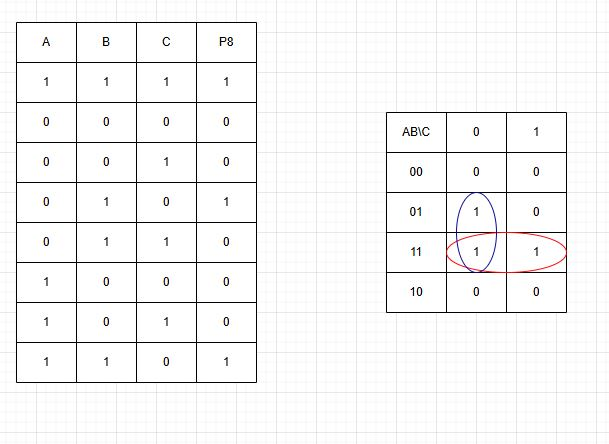
\includegraphics[width=.9\linewidth]{../../CW0POPRW/P8.JPG}
\caption{Tablica Karnaugh dla funkcji \(P_8\) i \(P_{11}\)}
\end{figure}
\begin{figure}[H]
\centering
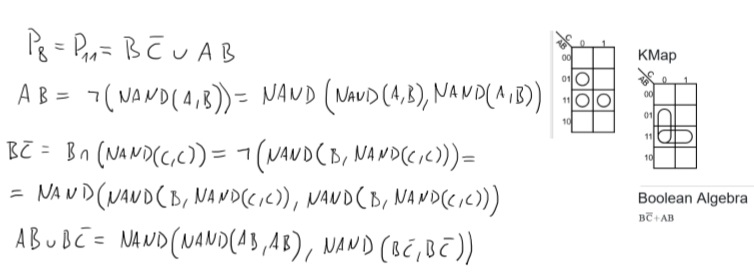
\includegraphics[width=.9\linewidth]{p8p11.jpg}
\caption{Przekształcenia dla funkcji \(P_8\) i \(P_{11}\)}
\end{figure}

\begin{figure}[H]
\centering
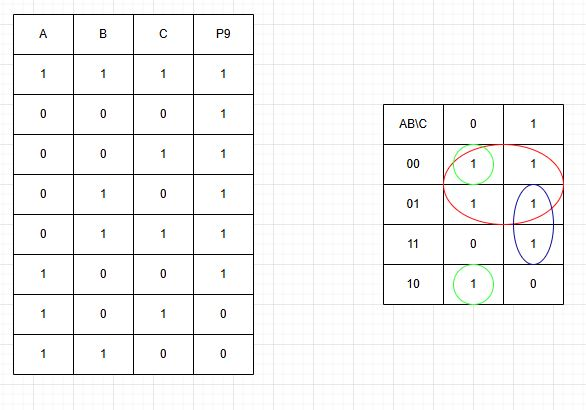
\includegraphics[width=.9\linewidth]{../../CW0POPRW/P9.JPG}
\caption{Tablica Karnaugh dla funkcji \(P_9\) i \(P_{10}\)}
\end{figure}
\begin{figure}[H]
\centering
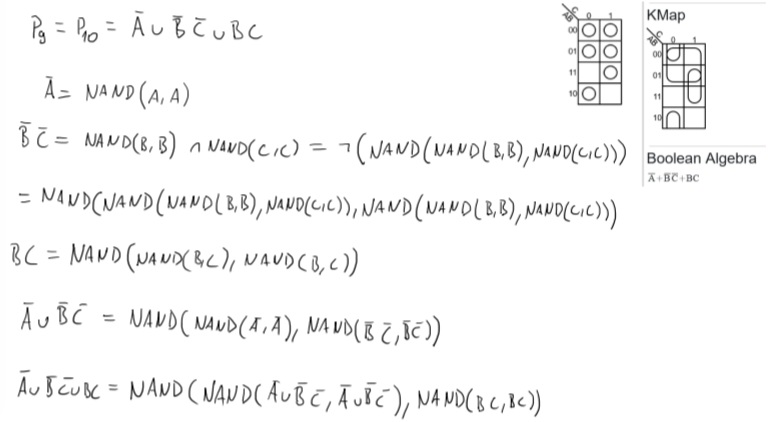
\includegraphics[width=.9\linewidth]{p9p10.jpg}
\caption{Przekształcenia dla funkcji \(P_9\) i \(P_{10}\)}
\end{figure}

\begin{figure}[H]
\centering
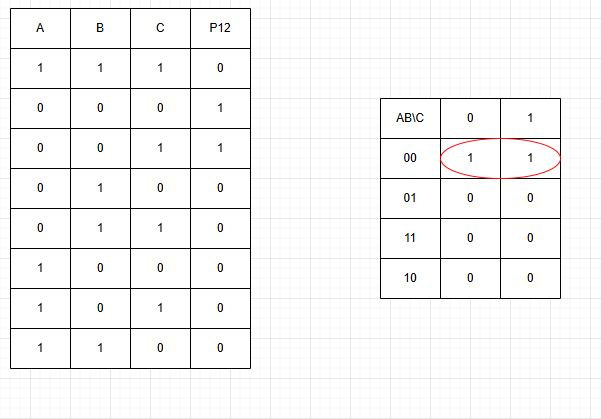
\includegraphics[width=.9\linewidth]{../../CW0POPRW/P12.JPG}
\caption{Tablica Karnaugh dla funkcji \(P_{12}\) i \(P_{15}\)}
\end{figure}
\begin{figure}[htbp]
\centering
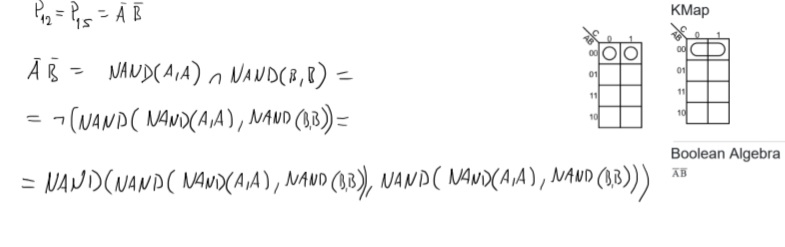
\includegraphics[width=.9\linewidth]{p12p15.jpg}
\caption{Przekształcenia dla funkcji \(P_{12}\) i \(P_{15}\)}
\end{figure}

\begin{figure}[H]
\centering
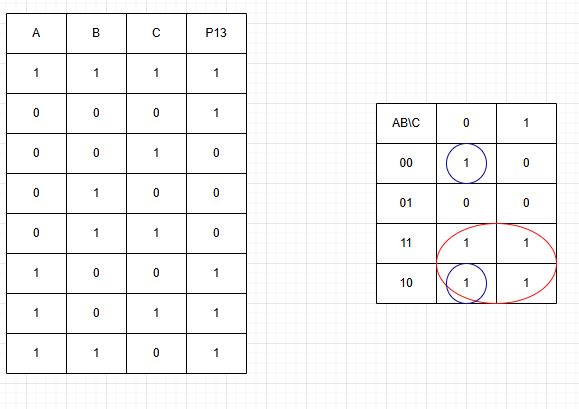
\includegraphics[width=.9\linewidth]{../../CW0POPRW/P13.JPG}
\caption{Tablica Karnaugh dla funkcji \(P_{13}\) i \(P_{14}\)}
\end{figure}
\begin{figure}[H]
\centering
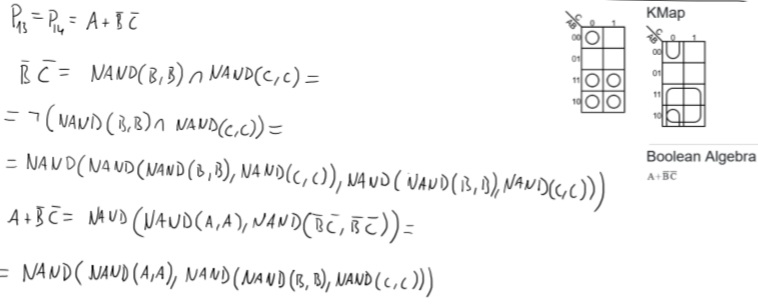
\includegraphics[width=.9\linewidth]{p13p14.jpg}
\caption{Przekształcenia dla funkcji \(P_{13}\) i \(P_{14}\)}
\end{figure}

\begin{figure}[H]
\centering
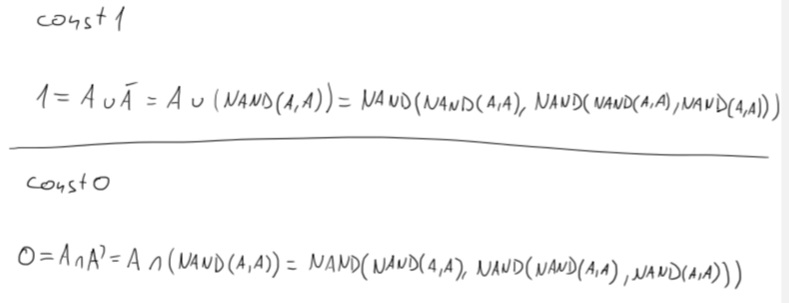
\includegraphics[width=.9\linewidth]{const.jpg}
\caption{Przekształcenia dla funkcji stałych}
\end{figure}

Jak można zaobserwować na rysunkach 3-7 zredukowane formy, przy użyciu odpowiednich praw logiki, przekształciliśmy na wzory
wykorzystujące wyłącznie bramki NAND, gotowe do zastosowania w budowie finalnego układu.
\section{Schemat układu}
\label{sec:org255dea5}

Korzystając z wyprowadzonych na rysunkach 3-7 wzorów na sygnały wyjściowe, byliśmy gotowi aby stworzyć schemat układu w programie \texttt{Multisim}.

\begin{figure}[H]
\centering
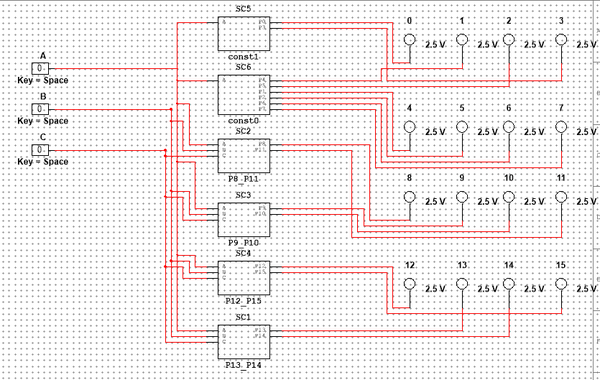
\includegraphics[width=.9\linewidth]{uklad.png}
\caption{Schemat układu z podziałem na bramki w programie \texttt{Multisim}}
\end{figure}

\begin{figure}[H]
\centering
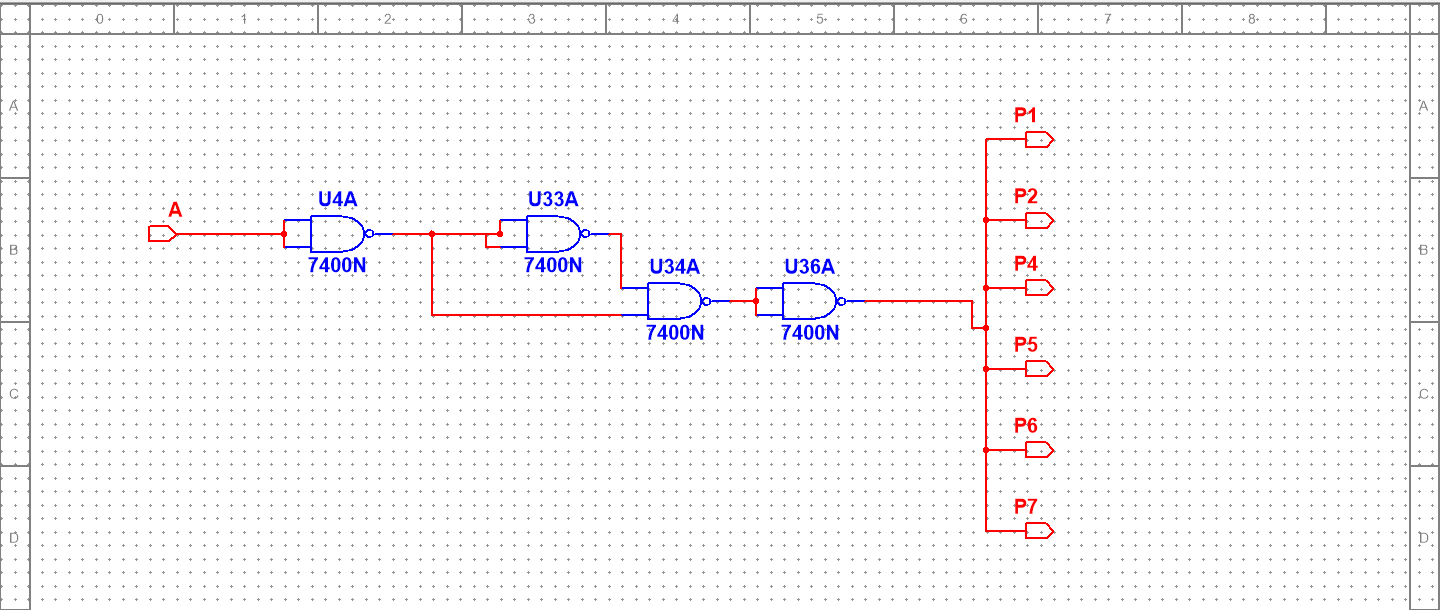
\includegraphics[width=.9\linewidth]{p1p7m.png}
\caption{Bramka odpowiedzialna za sygnały wyjściowe \(P_1\) do \(P_7\)}
\end{figure}

\begin{figure}[H]
\centering
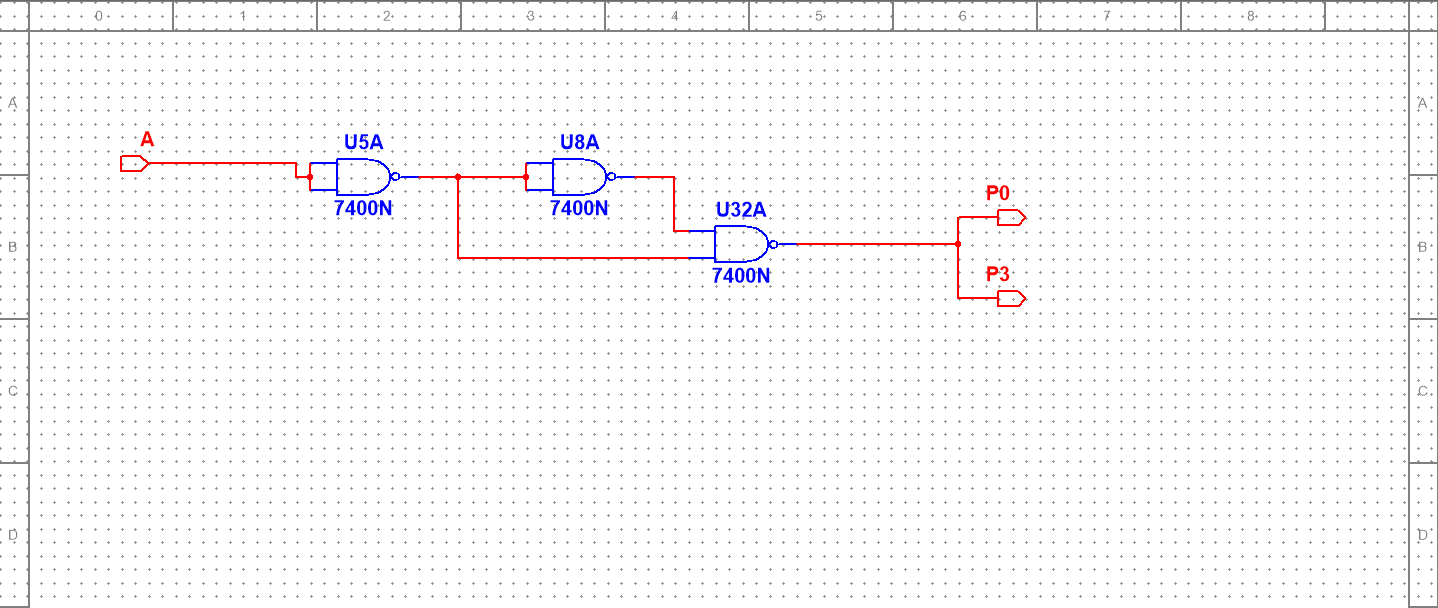
\includegraphics[width=.9\linewidth]{p0p3m.png}
\caption{Bramka odpowiedzialna za sygnały wyjściowe \(P_0\) oraz \(P_3\)}
\end{figure}

\begin{figure}[H]
\centering
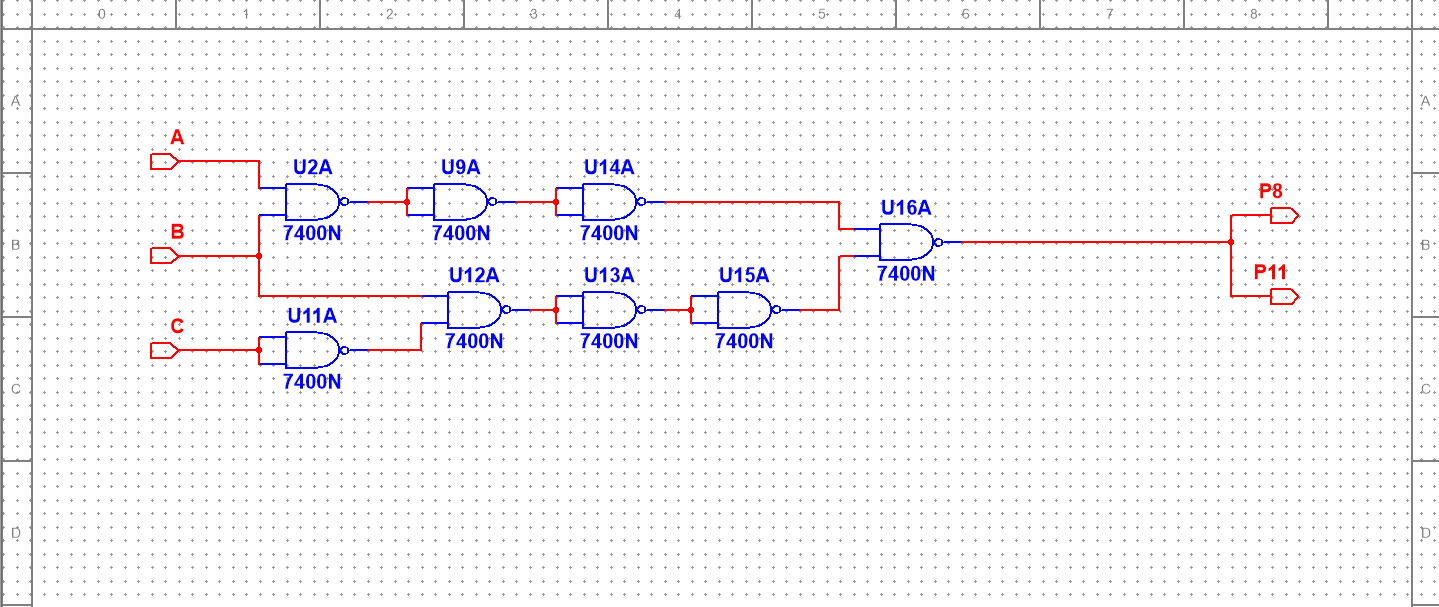
\includegraphics[width=.9\linewidth]{p8p11m.png}
\caption{Bramka odpowiedzialna za sygnały wyjściowe \(P_8\) oraz \(P_{11}\)}
\end{figure}

\begin{figure}[H]
\centering
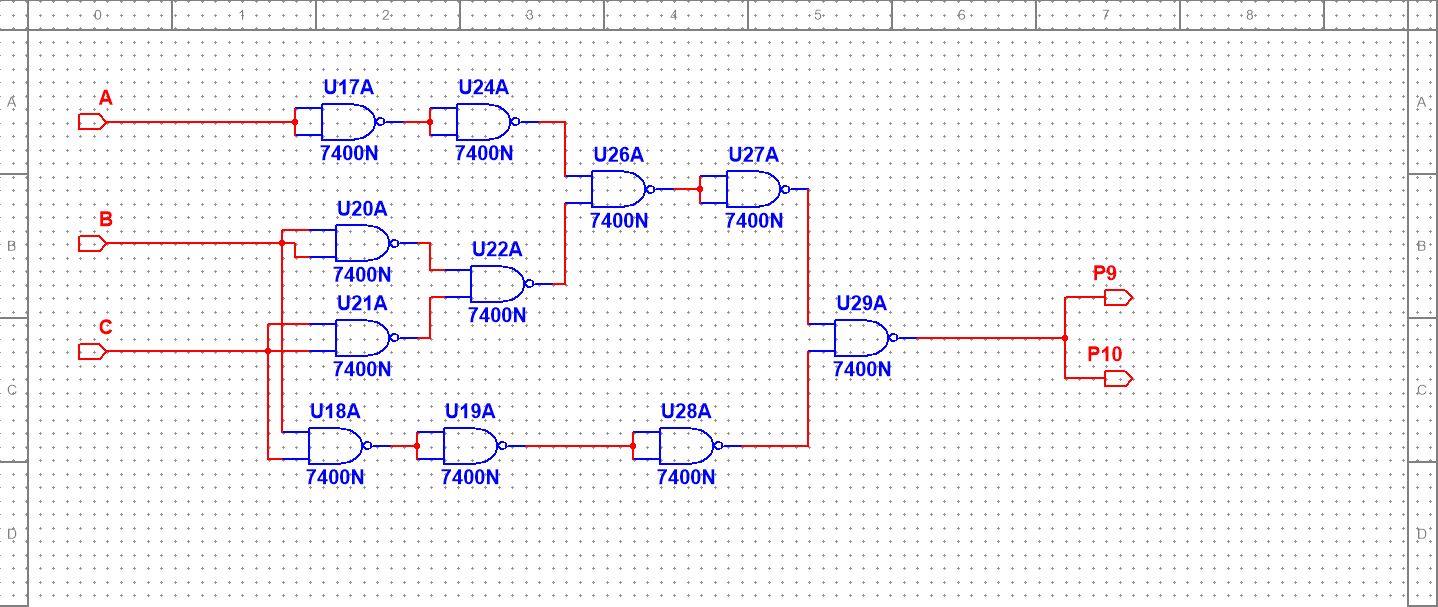
\includegraphics[width=.9\linewidth]{p9p10m.png}
\caption{Bramka odpowiedzialna za sygnały wyjściowe \(P_9\) oraz \(P_{10}\)}
\end{figure}

\begin{figure}[H]
\centering
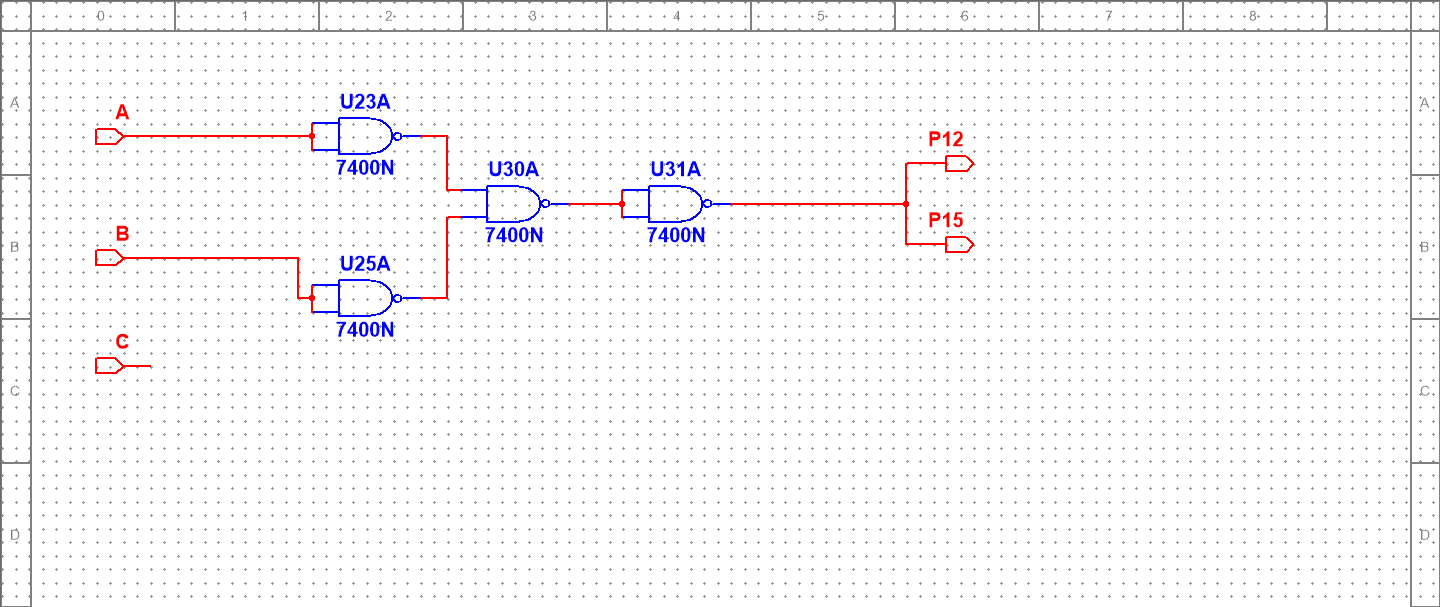
\includegraphics[width=.9\linewidth]{p12p15m.png}
\caption{Bramka odpowiedzialna za sygnały wyjściowe \(P_{12}\) oraz \(P_{15}\)}
\end{figure}

\begin{figure}[H]
\centering
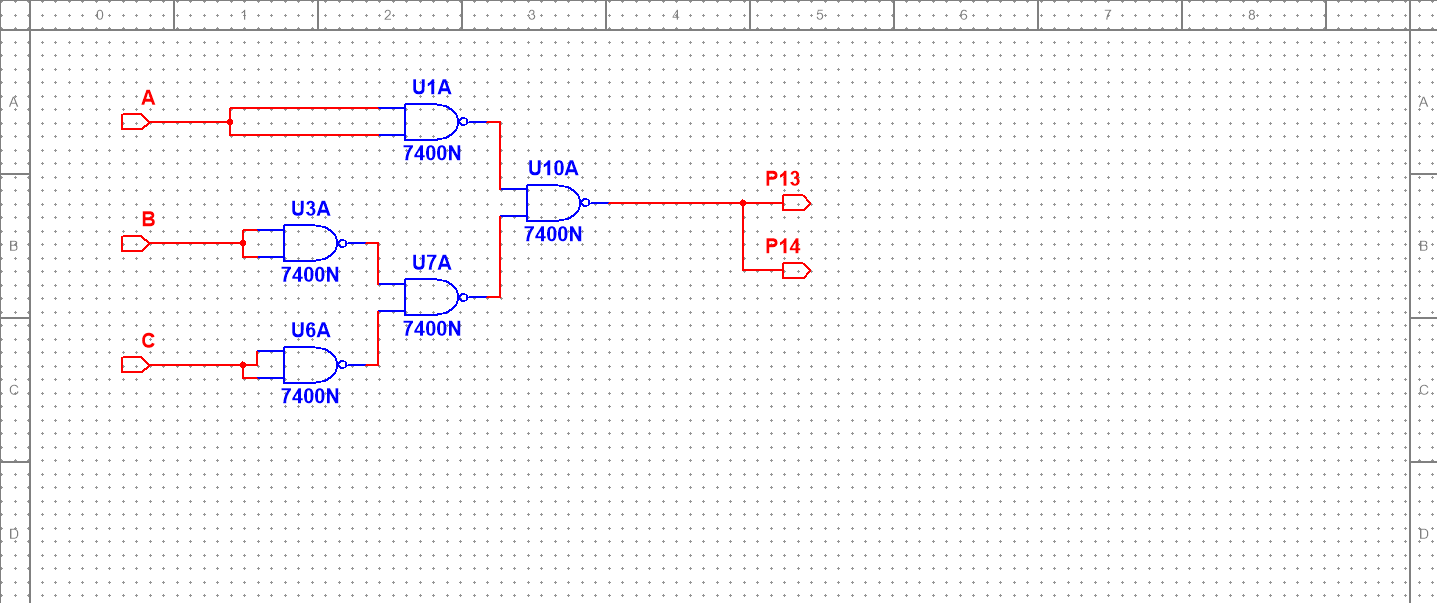
\includegraphics[width=.9\linewidth]{p13p14m.png}
\caption{Bramka odpowiedzialna za sygnały wyjściowe \(P_{13}\) oraz \(P_{14}\)}
\end{figure}
\section{Stanowisko testujące}
\label{sec:orga0bf1f2}

Układ testujący został zaprojektowany w celu automatycznej weryfikacji poprawności działania
głównego układu transkodera. Jego zadaniem jest porównywanie wyników generowanych przez
właściwy układ z wartościami referencyjnymi, uzyskanymi z równolegle działającego testera. Składa się
on z następujących elementów:

\begin{itemize}
\item Generator słów (XWG1) – generuje wszystkie możliwe kombinacje sygnałów wejściowych A,
B, C (od 000 do 111). Sygnały te są jednocześnie podawane do testowanego układu transkodera
oraz do układu testującego, co zapewnia synchroniczne porównanie wyników.

\item Tester (subcircuit o nazwie „Tester”) – zbudowany został z 8 sekcji, z których każda odpowiada
jednej z możliwych kombinacji wejść A, B, C. Każda sekcja zawiera osobny zestaw bramek
NAND, które na podstawie ustalonej logiki generują oczekiwane wyjście dla danej kombinacji.
Wyjścia z poszczególnych sekcji są następnie łączone przy użyciu bramek AND oraz OR w taki
sposób, aby zapewnić, że w danym momencie aktywna jest tylko jedna sekcja – dokładnie ta,
która odpowiada aktualnemu stanowi wejść. Dzięki temu można w pełni dynamicznie
odwzorować prawidłowe działanie transkodera bez potrzeby ręcznej zmiany konfiguracji.

\item Bramki XOR (7486) – do każdego z 16 wyjść podłączona jest bramka XOR, która porównuje
sygnał wyjściowy z transkodera z odpowiednim wyjściem z układu testującego. Jeśli wartości
się różnią, oznacza to błąd – wtedy zapala się odpowiednia dioda LED.

\item XLA1 (Logic Analyzer) – pełni rolę pomocniczą i umożliwia obserwację przebiegów logicznych
w czasie rzeczywistym. Pozwala to na dokładniejszą analizę pracy całego układu oraz
identyfikację ewentualnych problemów.

\item Wyświetlacz siedmiosegmentowy (HEX) – połączony z wejściami A, B i C za pośrednictwem
układu dekodera 7447N, wyświetla aktualną kombinację testowaną przez układ (w postaci
liczby binarnej od 000 do 111), co umożliwia łatwe śledzenie, który przypadek jest aktualnie
sprawdzany.
\end{itemize}

Dzięki zastosowaniu generatora słów i automatycznego testera możliwe jest szybkie i powtarzalne
testowanie wszystkich możliwych wejść bez ingerencji użytkownika. Układ reaguje natychmiastowo na
każdą nieprawidłowość, co znacznie przyspiesza proces weryfikacji poprawności działania transkodera.

\begin{figure}[H]
\centering
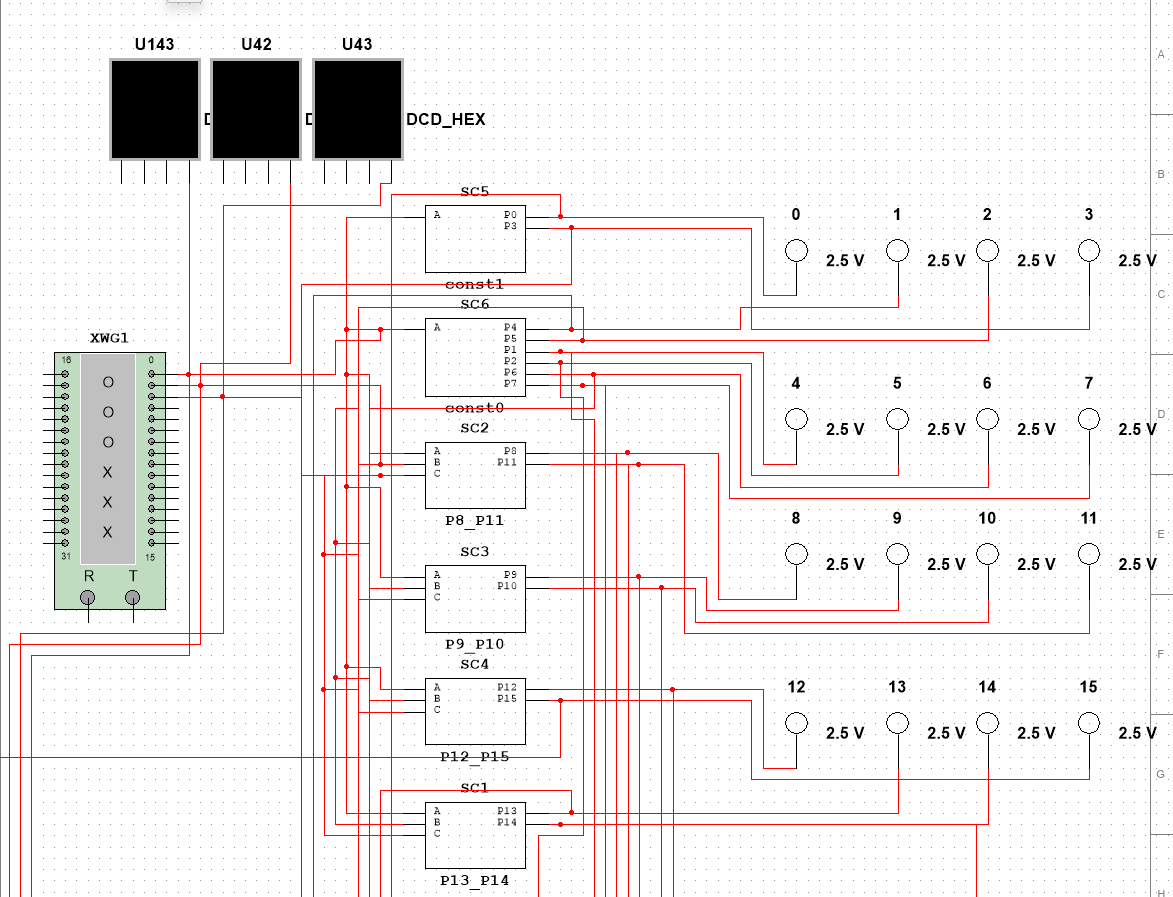
\includegraphics[width=.9\linewidth]{../uklad_testujacy_cw0_gora.png}
\caption{Układ testujący (dalsza część niżej)}
\end{figure}
\begin{center}
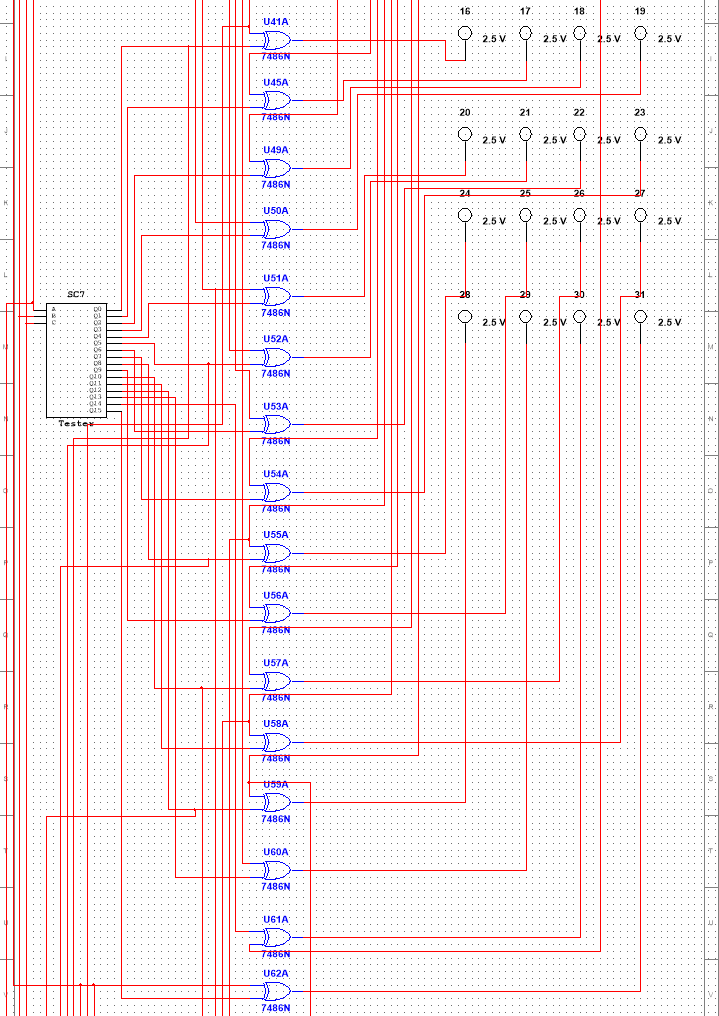
\includegraphics[width=.9\linewidth]{../uklad_testujacy_cw0_srodek.png}
\end{center}
\begin{center}
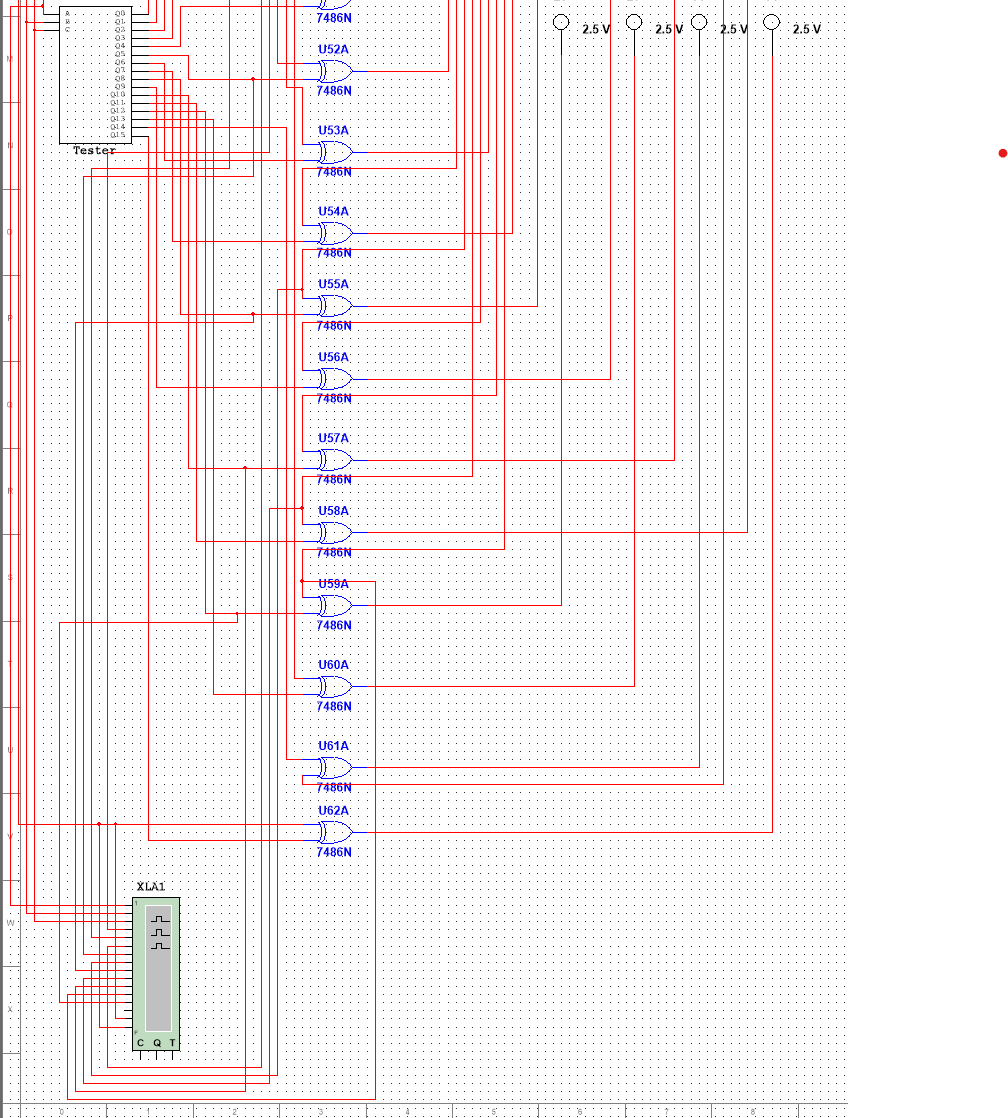
\includegraphics[width=.9\linewidth]{../uklad_testujacy_cw0_dol.png}
\end{center}
\section{Podsumowanie oraz wnioski}
\label{sec:org39466c6}

Kluczowym etapem ćwiczenia była minimalizacja funkcji logicznych przy użyciu tablic Karnaugh, a następnie przekształcenie
wszystkich wyrażeń do formy realizowalnej wyłącznie bramkami NAND, stosując prawa logiki i przekształcenia algebraiczne.
Wykonanie tego etapu w pierwszej kolejności uprościło znacznie stworzenie schematu układu, umożliwiając zbudowanie w programie \texttt{Multisim}
i przetestowanie jego finalnej wersji bez konieczności tworzenia bardziej złożonych prototypów. Słabą stroną tego podejścia jest brak możliwości wykrycia
błędów na wczesnym etapie projektowania, potencjalnym rozwiązaniem tego problemu byłyby np. programistyczne testy logiki poszczególnych bramek, co z kolei
dodatkowo skomplikowałoby proces weryfikacji działania.

\bigskip

Praktyczne zastosowania zaprojektowanego układu obejmują:
\begin{itemize}
\item Systemy wyświetlania prostych ikon w urządzeniach o niskiej rozdzielczości (np. wyświetlacze LED).
\item Urządzenia mające charakter informacji publicznej, gdzie przełamanie bariery językowej jest porządane, np. znaki ostrzegawcze, komunikaty o opóźnieniach, jakości powietrza itp.
\item Interfejsy użytkownika w układach embedded, np. w elektronice użytkowej lub zabawkowej.
\end{itemize}

\begin{figure}[H]
\centering
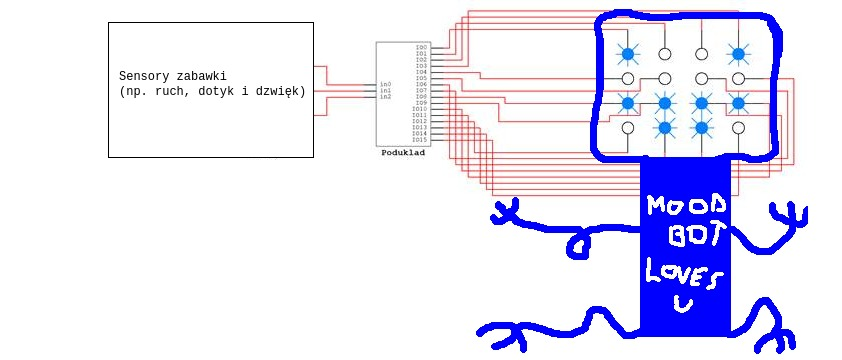
\includegraphics[width=.9\linewidth]{unholy_abomination.jpg}
\caption{Przykładowe zastosowanie układu}
\end{figure}

Układ stanowi przykład efektywnego wykorzystania podstawowych elementów logicznych do realizacji czytelnych funkcji wizualnych,
co może znaleźć zastosowanie w projektach wymagających prostoty i niskiego poboru mocy.
\end{document}
